\documentclass[dvipdfmx, twocolumn]{jsarticle}

\usepackage[version=3]{mhchem}
\usepackage{amsmath}
\usepackage[siunitx]{circuitikz}
\usepackage{graphicx}
\usepackage{here}

\setlength\parindent{0pt}

\begin{document}
\title{制御工学第一レポート}
\author{03190449  堀 紡希}
\date{\ 7月17日}
\maketitle

\section{基本課題}

\subsection{Bode線図の折れ線近似}

$P_{1}(s)=\frac{1}{s+100}$

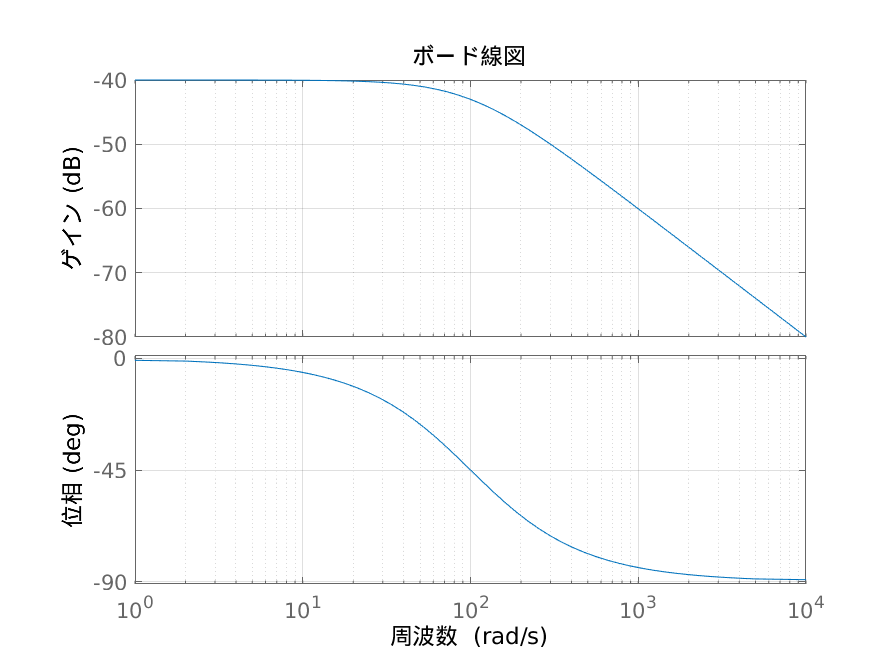
\includegraphics[scale = 0.5]{bode1.png}

$P_{2}(s)=\frac{s}{s+100}$

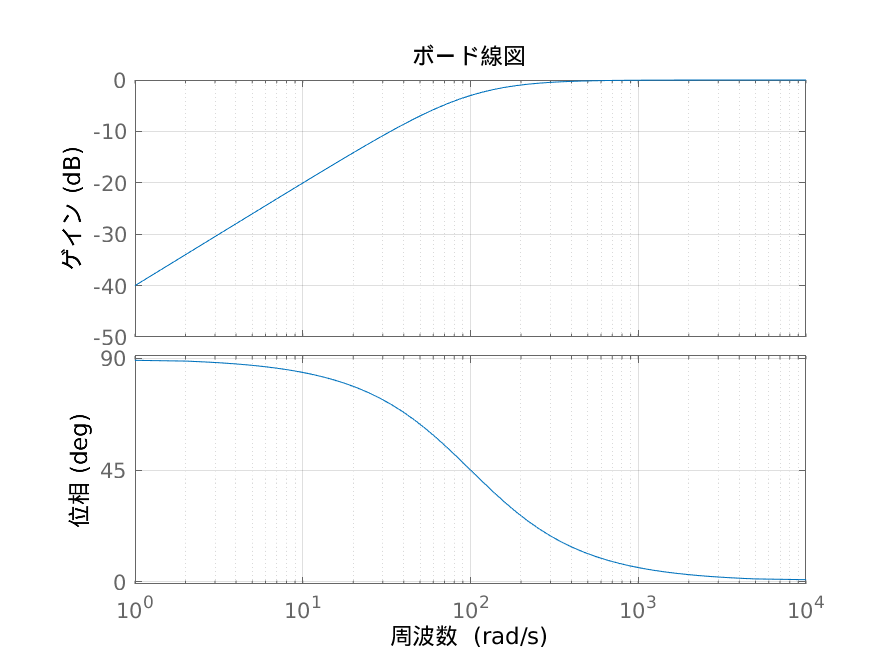
\includegraphics[scale = 0.5]{bode2.png}

\subsection{根軌跡}

MATLABで描いた$P_{3}(s) = \frac{1}{(s+2)(s^{2}+2s+2)}$の根軌跡は以下の通り

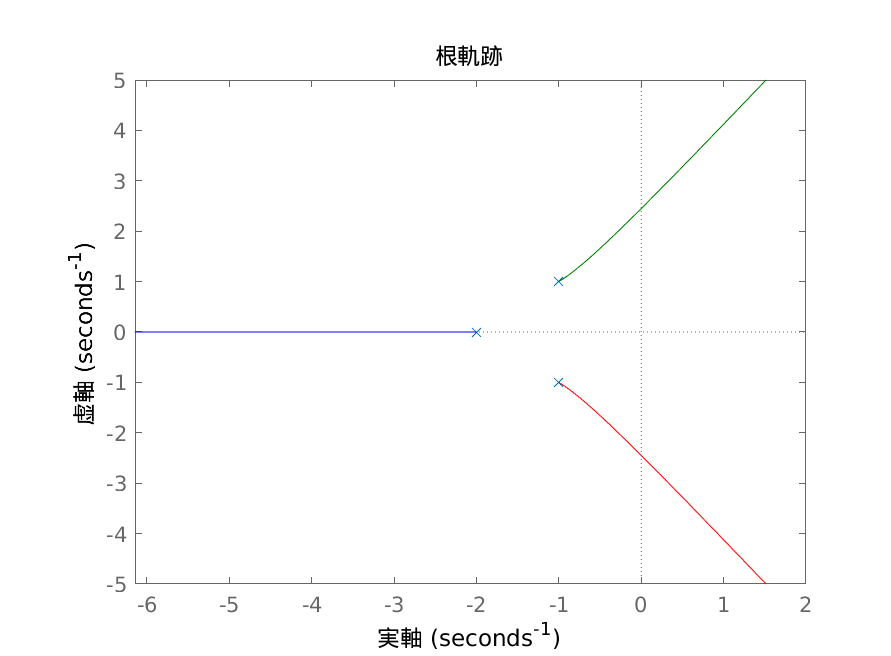
\includegraphics[scale = 0.5]{rlocus.png}


根軌跡のそれぞれの性質について、

\begin{enumerate}
\item 軌跡の数は次数と同じで3本

\item 極$-2, -1\pm j$から出発し、零点は存在しないので3本全てが無限遠点に発散する

\item 軌跡は実軸対称である

\item 実軸上の点で、その右側に極が奇数個あれば、その点は軌跡上の点となっている

\item 無限遠点に至る軌跡の漸近線の角度は$\frac{180^{\circ}+360^{\circ}}{3} = 60^{\circ}, 180^{\circ}, 300^{\circ}$

\item 漸近線と実軸の交点はただひとつ、$((-1)+(-1+j)+(-1-j))/3 = -4/3$である

\item 虚軸を横切る点
\end{enumerate}
\subsection{ステップ応答}

1)MATLABによるステップ応答

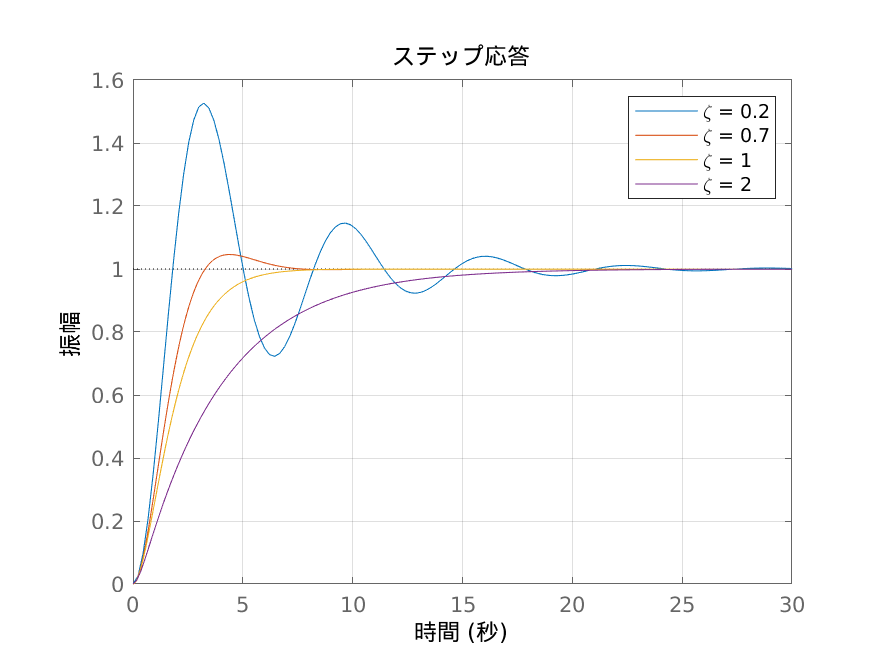
\includegraphics[scale = 0.5]{3(1).png}


2)逆ラプラス変換によって求めた解

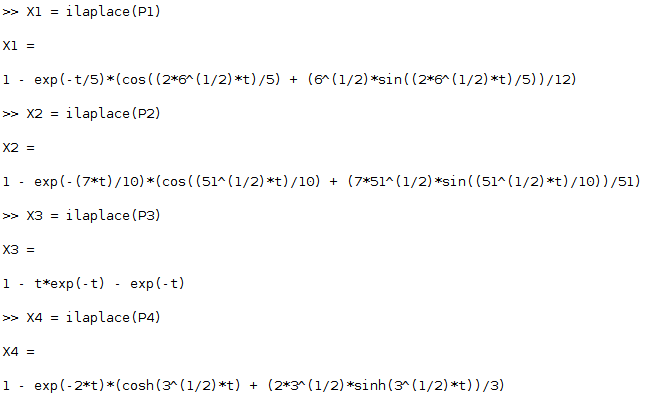
\includegraphics[scale=0.3]{Sc.png}

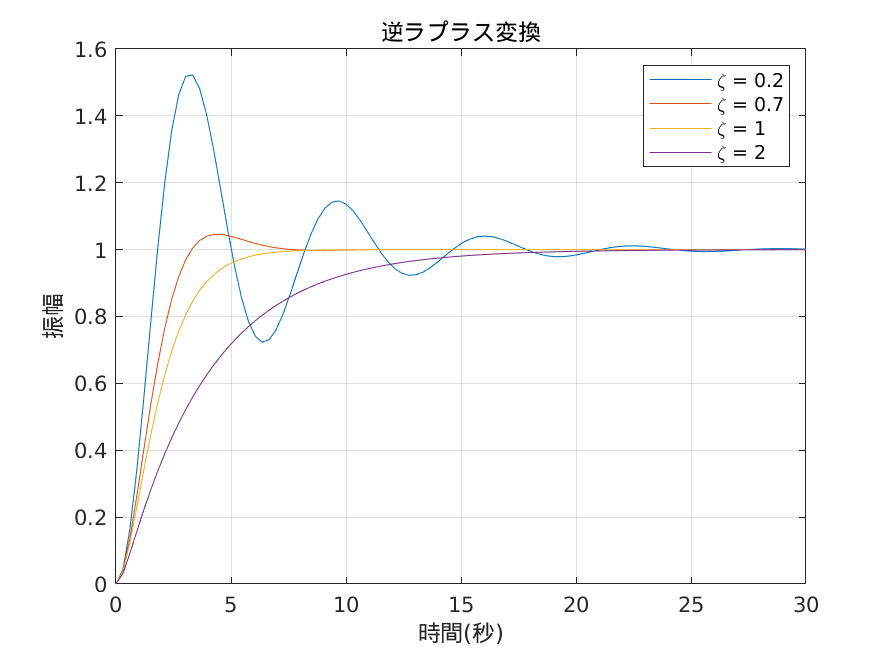
\includegraphics[scale = 0.5]{3(2).png}

\section{応用課題}

\subsection{制御対象のモデル化}

mn=4.2,bn=80,kn=2500,として制御対象をモデル化することができた。

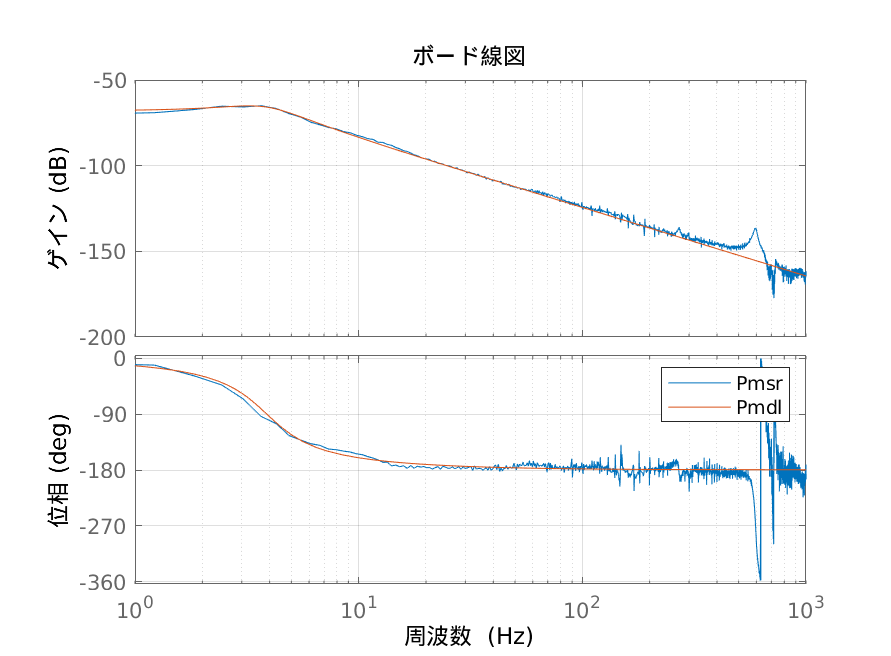
\includegraphics[scale=0.5]{4.png}

\end{document}